\documentclass{article}
\usepackage[margin=2cm]{geometry}
\usepackage{tabu}
\usepackage{mathtools}
\usepackage{enumitem}
\usepackage{amssymb}
\usepackage{newcent}
\usepackage{amsmath}
\usepackage{subcaption}
\usepackage{graphics}
\usepackage{hyperref}


\title{COL726 Homework 4}
\author{Lovish Madaan \\ \texttt{2015CS50286}}
\date{}
\begin{document}
\maketitle

\begin{enumerate}
    \item Since $A$ is diagonal, we have:
    \begin{equation}
    \lambda_1 = a_{11} \qquad \& \qquad \lambda_2 = a_{22}
    \label{q1:1}
    \end{equation}
    Since the eigenvectors remain normalized under perturbation i.e. $||q_1 + \delta q_1||_2 = 1$, using this along with the fact that $q_1^Tq_1 = 1$, we have
    $$||q_1 + \delta q_1||_2^2 = (q_1 + \delta q_1)^T(q_1 + \delta q_1) = 1$$
    $$1 +  q_1^T\delta q_1 + \delta q_1^Tq_1 + \delta q_1^T\delta q_1 = 1$$
    $$q_1^T\delta q_1 + \delta q_1^Tq_1 \approx 0 \Rightarrow 2q_1^T\delta q_1 \approx 0$$
    Or simply,
    \begin{equation}
    q_1^T\delta q_1 = 0
    \label{q1:2}
    \end{equation}
    If we write $\delta q_1$ as $\begin{bmatrix}
        \delta q_{11} \\
        \delta q_{21} \\
    \end{bmatrix}$, using $q_1 = \begin{bmatrix}
        1\\
        0\\
    \end{bmatrix}$, we get
    \begin{equation}
    \delta q_{11} = 0
    \label{q1:3}
    \end{equation}
    Let the perturbed eigenvalue corresponding to the eigenvector $q_1 + \delta q_1$ be $\lambda_1 + \delta \lambda_1$. We then have
    $$(A + \delta A)(q_1 + \delta q_1) = (\lambda_1 + \delta \lambda_1)(q_1 + \delta q_1)$$
    Since $Aq_1 = \lambda_1q_1$, we get
    $$A\delta q_1 + \delta Aq_1 + \delta A\delta q_1 = \lambda_1\delta q_1 + \delta \lambda_1q_1 + \delta\lambda_1\delta q_1$$
    Dropping the second order terms and replacing the approximation with equality, we get
    \begin{equation}
    A\delta q_1 + \delta Aq_1 = \lambda_1\delta q_1 + \delta\lambda_1q_1
    \label{q1:4}
    \end{equation}
    Multiply equation \ref{q1:4} with $q_1^T$ to get
    $$q_1^TA\delta q_1 + q_1^T\delta Aq_1 = \lambda_1q_1^T\delta q_1 + \delta\lambda_1q_1^Tq_1$$
    Using equations \ref{q1:2} and \ref{q1:3}, we have
    $$\begin{bmatrix}
        1 & 0\\
    \end{bmatrix}\begin{bmatrix}
        a_{11} & 0\\
        0 & a_{22}\\
    \end{bmatrix}\begin{bmatrix}
        0\\
        \delta q_{21}\\
    \end{bmatrix} + \begin{bmatrix}
        1 & 0\\
    \end{bmatrix}\begin{bmatrix}
        \delta a_{11} & \delta a_{12}\\
        \delta a_{21} & \delta a_{22}\\
    \end{bmatrix}\begin{bmatrix}
        1\\
        0\\
    \end{bmatrix} = 0 + \delta \lambda_1$$
    Therefore,
    \begin{equation}
    \delta\lambda_1 = 0 + \delta a_{11} = \delta a_{11}
    \label{q1:5}
    \end{equation}
    Put the values obtained in equations \ref{q1:1}, \ref{q1:3} and \ref{q1:5} in the equation \ref{q1:4} to get
    $$\begin{bmatrix}
        a_{11} & 0\\
        0 & a_{22}\\
    \end{bmatrix}\begin{bmatrix}
        0\\
        \delta q_{21}\\
    \end{bmatrix} + \begin{bmatrix}
        \delta a_{11} & \delta a_{12}\\
        \delta a_{21} & \delta a_{22}\\
    \end{bmatrix}\begin{bmatrix}
        1\\
        0\\
    \end{bmatrix} = a_{11}\begin{bmatrix}
        0\\
        \delta q_{21}\\
    \end{bmatrix} + \delta a_{11}\begin{bmatrix}
        1\\
        0\\
    \end{bmatrix}$$
    $$\begin{bmatrix}
        0\\
        \delta q_{21}(a_{22} - a_{11})\\
    \end{bmatrix} = \begin{bmatrix}
        0\\
        -\delta a_{21}\\
    \end{bmatrix}$$
    Therefore using equation \ref{q1:1},
    $$\delta q_1 = \begin{bmatrix}
        \delta q_{11}\\
        \delta q_{21}\\
    \end{bmatrix} = \begin{bmatrix}
        0\\
        \frac{-\delta a_{21}}{a_{22} - a_{11}}\\
    \end{bmatrix} = \begin{bmatrix}
        0\\
        \frac{\delta a_{21}}{\lambda_1 - \lambda_2}
    \end{bmatrix}$$
    When $\lambda_1 \approx \lambda_2$, we have $||\delta q_1|| = \frac{|\delta a_{21}|}{|\lambda_1 - \lambda_2|} >> 0$. Hence, the eigenvectors are ill-conditioned when the eigenvalues are close to each other.
    \item \begin{enumerate}[label=(\alph*)]
    \item Updating Algorithm 10.1 of Trefethen \& Bau for an upper Hessenberg Matrix($H = QR$) results in:
    \begin{enumerate}
        \item for $k = 1$ to $m - 1$
        \item $\qquad$ $x = H_{k : k + 1, k}$
        \item $\qquad$ $v_k = sign(x_1)||x||_2e_1 + x$
        \item $\qquad$ $v_k = v_k / ||v_k||_2$
        \item $\qquad$ $H_{k : k + 1, k : m} = H_{k : k + 1, k : m} - 2v_k(v_k^TH_{k : k + 1, k : m})$
        \item $v_m = sign(H_{m, m})$
        \item $H_{m, m} = -H_{m, m}$
    \end{enumerate}
    $H$ is modified in place and the resultant is R. $v_1, \cdots, v_m$ are the modified reflection vectors. To get the reflection vectors as specified in the book($v_k^b$), append zeros at the end of vector $v_k$, i.e. $v_k^b = [v_k;zeros(min(m - k - 1, 0))]$ . Now, in the for loop, steps \romannumeral 2 $\;$ - \romannumeral 4 $\;$ take constant time - $O(1)$. Step \romannumeral 5 $\;$ takes atmost $O(m)$ time per iteration. Therefore total time taken is $O(m * m) = O(m^2)$
    \item Now, suppose we have $(m + 1) \times (m + 1)$ upper Hessenberg matrix $H'$ as follows:
    $$H' = \begin{bmatrix}
        H & p\\
        q^T & r\\
    \end{bmatrix}$$
    where $p$ and $q$ are $m$ dimensional vectors and r is a scalar. Also, $q$ is of the form $\begin{bmatrix}
        0\\
        \vdots\\
        0\\
        q_m
    \end{bmatrix}$.\\
    In the algorithm above, $v_1, v_2, \cdots, v_{m - 1}$ are not modified for the QR factorization of $H'$($H' = Q'R'$). Also, if you look at step \romannumeral 5, it can be written as $H_{k : k + 1, i} = H_{k : k + 1, i} - 2(v_kv_k^T)H_{k : k + 1, i}$ for each column $i$. Hence the QR factorization of $H'$ is identical to QR factorization of $H$ for first $m - 1$ columns. So, the update rule i.e. step \romannumeral 5 $\;$ is to be performed only for columns $m$ and $m + 1$.\\
    Now, first construct $H' = \begin{bmatrix}
        R & p\\
        q^T & r\\
    \end{bmatrix}$ where $p,q,r$ are defined above and $R$ is obtained from the QR factorization of $H$. Note that $\{m, m\}$ element of $R$ is updated as $R_{m, m} = -R_{m ,m}$ before putting in $H'$.
    The entire algorithm is stated below:
    \begin{enumerate}
        \item for $k = 1$ to $m - 1$
        \item $\qquad$ $v'_k = v_k$
        \item $\qquad$ $H'_{k : k + 1, m + 1} = H'_{k : k + 1,m + 1} - 2v'_k(v_k'^TH'_{k : k + 1, m + 1})$
        \item $x = H'_{m : m + 1, m}$
        \item $v'_m = sign(x_1)||x||_2e_1 + x$
        \item $v'_m = v'_m / ||v'_m||_2$
        \item $H'_{m : m + 1, m : m + 1} = H'_{m : m + 1, m : m + 1} - 2v'_m(v_m'^TH'_{m : m + 1, m : m + 1})$
        \item $v_{m + 1} = sign(H'_{m + 1, m + 1})$
        \item $H'_{m + 1, m + 1} = -H'_{m + 1, m + 1}$
    \end{enumerate}
    The resultant $H'$ is $R'$. Step \romannumeral 3 $\;$ takes $O(1)$ time per iteration. Therefore total time for steps \romannumeral 1 $\;$ - \romannumeral 3 $\;$ is $O(m)$. Steps \romannumeral 4 $\;$ - \romannumeral 9 $\;$ take $O(1)$ time. So total time for entire algorithm is $O(m)$.
    \end{enumerate}
    \clearpage
    \item Suppose $v$ be an eigenvector of $A$ with corresponding eigenvalue $\lambda$. We have
    $$Av = \lambda v \Rightarrow A^{-1}Av = \lambda A^{-1}v \Rightarrow A^{-1}v = \frac{1}{\lambda}v$$
    Therefore, $A^{-1}$ has eigenvector $v$ with the corresponding eigenvalue $\frac{1}{\lambda}$.\\
    Also, since $A$ is non-singular and symmetric, $A$ has real eigenvalues and a complete set of orthonormal eigenvectors. Let the eigenvalues of $A$ be $\lambda_1, \cdots, \lambda_m$ and the corresponding eigenvectors be $u_1, \cdots, u_m$. Without loss of generality, assume that
    $$|\lambda_m| > \cdots > |\lambda_1|$$.
    \begin{enumerate}[label=(\alph*)]
    \item Now, algorithm 27.1 in Trefethen \& Bau(Power Iteration) gives the eigenvector corresponding to the largest eigenvalue of $A$ in absolute terms. Also,
    $$v^* = \{v | Av = \lambda_{min}^A v\} = \{v | A^{-1}v = \frac{1}{\lambda_{min}^A}v\} = \{v | A^{-1}v = \lambda_{max}^{A^{-1}}v\}$$.
    So, we will apply power iteration on $A^{-1}$ to get the eigenvector corresponding to maximum eigenvalue of $A^{-1}$. Let the black box be treated as functions $f$ and $f^{-1}$ on some vector $x$, i.e. $f(x) = Ax$ and $f^{-1}(x) = A^{-1}x$ respectively. Power Iteration algorithm is detailed below using the black box:
    \begin{enumerate}
        \item $v^{(0)} = $ some vector with $||v_0|| = 1$
        \item for $k = 1, 2, \cdots$
        \item $\qquad$ $w = f^{-1}(v^{(k - 1)})$
        \item $\qquad$ $v^{(k)} = w / ||w||$
    \end{enumerate}
    $v^{(k)}$ converges to either $u_1$ or $-u_1$, i.e. $v^{(k)} = \pm u_1$.
    \item The $k^{th}$ smallest eigenvalue of $A$ in absolute terms is $\lambda_k$. Therefore, $\frac{1}{\lambda_k}$ is the $k^{th}$ largest eigenvalue of $A^{-1}$ in absolute terms. Now, we will use Simultaneous Iteration(Algorithm 28.3 Trefethen \& Bau) to get the eigenvector corresponding to $k^{th}$ largest eigenvalue of $A^{-1}$($k^{th}$ smallest eigenvalue of $A$).
    \begin{enumerate}
        \item Pick $\hat{Q}^{(0)} \in \mathbb{R}^{m \times k}$ with orthonormal columns $q_1^{(0)}, \cdots, q_k^{(0)}$.
        \item for $i = 1, 2, \cdots$
        \item $\qquad$ $Z = \begin{bmatrix}
            f^{-1}(q_1^{i - 1}) & \cdots & f^{-1}(q_k^{i - 1})\\
        \end{bmatrix}$
        \item $\qquad$ $\hat{Q}^{(i)}\hat{R}^{(i)} = Z$ $\qquad$ reduced QR factorization of Z
    \end{enumerate}
    The vectors $q_1^{(i)}, \cdots, q_k^{(i)}$ converge to $\pm u_1, \cdots, \pm u_k$ respectively. And $u_k$ is the eigenvector corresponding to $k^{th}$ largest eigenvalue of $A^{-1}$($k^{th}$ smallest eigenvalue of $A$). Step \romannumeral 3 $\;$ takes $O(mk)$ time(copying the vectors to the matrix Z). Step \romannumeral 4 $\;$ is the reduced QR factorization, which can be computed using modified Gram-Schmidt orthogonalization in $O(2mk^2)$ time(Modified Gram-Schmidt gives $\hat{Q}$ directly). Therefore, total time taken is $O(mk^2)$.
    \end{enumerate}
    \clearpage
    \item If two matrices have the same characteristic polynomial, they have same eigenvalues since the roots of the characteristic polynomial are the eigenvalues. Let the characteristic polynomial of a matrix $A$ be denoted as $p_A(\lambda)$. We have
    $$p_A(\lambda) = det(A - \lambda I) = det((A - \lambda I)^T) = det(A^T - \lambda I^T) = det(A^T - \lambda I) = p_{A^T}(\lambda)$$
    Therefore, the eigenvalues of $A$ and $A^T$ are same.\\
    For an orthogonal matrix $Q$, we have $Q^TQ = QQ^T = I \Rightarrow Q^T = Q^{-1}$. Now, let
    $$X = Q^TAQ = Q^{-1}AQ = \begin{bmatrix}
        A_{11} & A_{12}\\
        \mathbf{0} & A_{22}\\
    \end{bmatrix}$$
    Now,
    $$p_X(\lambda) = det(Q^{-1}AQ - \lambda I) = det(Q^{-1}(A - \lambda I)Q) = det(Q^{-1})det(A - \lambda I)det(Q) = det(A - \lambda I) = p_A(\lambda)$$
    Therefore $X$ and $A$ have the same eigenvalues.
    Now, suppose $v$ be any $n$ dimensional eigenvector of $A_{11}$ with eigenvalue $\lambda$. Define $v' = \begin{bmatrix}
        v\\
        \mathbf{0}\\
    \end{bmatrix}$. $v'$ is $m$ dimensional. We have,
    $$Xv' = \begin{bmatrix}
        A_{11} & A_{12}\\
        \mathbf{0} & A_{22}\\
    \end{bmatrix}\begin{bmatrix}
        v\\
        \mathbf{0}\\
    \end{bmatrix} = \begin{bmatrix}
        A_{11}v + A_{12}\mathbf{0}\\
        \mathbf{0}v + A_{22}\mathbf{0}\\
    \end{bmatrix} = \begin{bmatrix}
        A_{11}v\\
        \mathbf{0}\\
    \end{bmatrix} = \lambda \begin{bmatrix}
        v\\
        \mathbf{0}\\
    \end{bmatrix} = \lambda v'$$
    Therefore $\lambda$ is an eigenvalue of $X$. Since, the choice of $v$ was arbitrary, the eigenvalues of $A_{11}$ are also eigenvalues of $X$. We proved that $X$ and $A$ have the same eigenvalues. Consequently, the eigenvalues of $A_{11}$ are also eigenvalues of $A$.\\
    Now, suppose $v$ be any $(m - n)$ dimensional eigenvector of $A_{22}^T$ with eigenvalue $\lambda$. Define $v' = \begin{bmatrix}
        \mathbf{0}\\
        v\\
    \end{bmatrix}$. $v'$ is $m$ dimensional. We have,
    $$X^Tv' = \begin{bmatrix}
        A_{11}^T & 0\\
        A_{12}^T & A_{22}^T\\
    \end{bmatrix}\begin{bmatrix}
        \mathbf{0}\\
        v\\
    \end{bmatrix} = \begin{bmatrix}
        A_{11}^T\mathbf{0} + \mathbf{0}v\\
        A_{12}^T\mathbf{0} + A_{22}^Tv\\
    \end{bmatrix} = \begin{bmatrix}
        \mathbf{0}\\
        A_{12}^Tv\\
    \end{bmatrix} = \lambda \begin{bmatrix}
        \mathbf{0}\\
        v\\
    \end{bmatrix} = \lambda v'$$
    Therefore $\lambda$ is an eigenvalue of $X^T$. Since, the choice of $v$ was arbitrary, the eigenvalues of $A_{22}^T$ are also eigenvalues of $X^T$. Since we proved that eigenvalues of any matrix $M$ and $M^T$ are same, we get that the eigenvalues of $A_{22}$ are also eigenvalues of $X$. We proved that $X$ and $A$ have the same eigenvalues. Consequently, the eigenvalues of $A_{22}$ are also eigenvalues of $A$.\\
    \item We have
    $$f(x) = p(x) = x^3 - x^2 - x + 1 = (x + 1)(x - 1)^2$$
    $$f'(x) = p'(x) = 3x^2 - 2x - 1 = (x - 1)(3x + 1)$$
    $$f''(x) = p''(x) = 6x - 2 = 2(3x - 1)$$
    \begin{enumerate}[label=(\alph*)]
        \item In Newton's method, we have
        \begin{equation}
        g(x) = x - \frac{f(x)}{f'(x)}
        \label{eq:newton}
        \end{equation}
        Therefore, the $(k + 1)^{th}$ iteration is given by:
        $$x_{k + 1} = g(x_k) = x_k - \frac{p(x_k)}{p'(x_k)} = x_k - \frac{x_k^3 - x_k^2 - x_k + 1}{3x_k^2 - 2x_k - 1}$$
        Now, the 4 iterations performed with $x_0 = -2$ and $x_0 = 2$ give the following iterates:
        \begin{center}
        \begin{tabular}{c | c | c}
        $\mathbf{x_0}$ & -2.00000 & 2.00000 \\
        \hline
        $x_1$ & -1.40000 & 1.57143 \\
        $x_2$ & -1.10000 & 1.31429 \\
        $x_3$ & -1.00870 & 1.16714 \\
        $x_4$ & -1.00008 & 1.08667 \\
        \end{tabular}
        \end{center}
        \item Given solution $x^*$, the error after $k^{th}$ iteration is given by
        $$e_{k + 1} = x_{k + 1} - x^* = g(x_k) - g(x^*)$$
        Using Taylor Series, we have
        $$e_{k + 1} = g(x_k) - g(x^*) = g'(x^*)(x_k - x^*) + g''(x^*)\frac{(x_k - x^*)^2}{2} + \cdots$$
        Using $e_k = x_k - x^*$,
        \begin{equation}
        e_{k + 1} = g'(x^*)e_k + g''(x^*)\frac{e_k^2}{2} + \cdots
        \label{q5:b}
        \end{equation}
        Now, using equation \ref{eq:newton},
        $$g'(x) = \frac{f(x)f''(x)}{(f'(x))^2} = \frac{2(x + 1)(3x - 1)}{(3x + 1)^2}$$
        For simple root $x^* = -1$, $g'(x^*) = 0$, therefore the rate of convergence is quadratic(from equation \ref{q5:b}):
        $$lim_{k \rightarrow \infty}\frac{|e_{k + 1}|}{|e_k|^2} = C = \frac{|g''(x^*)|}{2}$$
        For double root $x^* = 1$, $g'(x^*) = \frac{1}{2}$, therefore the rate of convergence is linear(from equation \ref{q5:b}):
        $$lim_{k \rightarrow \infty}\frac{|e_{k + 1}|}{|e_k|} = C = |g'(x^*)| = \frac{1}{2} = 0.5$$
        \item Let $f(x)$ be any arbitrary function with double root $a$. Therefore we can write $f(x)$ as $f(x) = (x - a)^2h(x)$. We have
        $$f'(x) = (x - a)^2h'(x) + 2(x - a)h(x) = (x - a)((x - a)h'(x) + 2h(x))$$
        $$f''(x) = ((x - a)h'(x) + 2h(x)) + (x - a)((x - a)h''(x) + h'(x) + 2h'(x))$$
        Now, since $g(x) = x - \frac{f(x)}{f'(x)}$, we get
        $$g'(x) = \frac{f(x)f''(x)}{(f'(x))^2} = \frac{(x - a)^2h(x)[(x - a)^2h''(x) + 4(x - a)h'(x) + 2h(x)]}{(x - a)^2((x - a)h'(x) + 2h(x))^2}$$
        \begin{equation}
        g'(a) = \frac{h(a)[2h(a)]}{(2h(a))^2} = \frac{1}{2} = 0.5
        \label{q5:c}
        \end{equation}
        Now, the rate of convergence starting from a point near $a$ is linear(from equation \ref{q5:b}):
        $$lim_{k \rightarrow \infty}\frac{|e_{k + 1}|}{|e_k|} = C = |g'(a)| = \frac{1}{2} = 0.5$$
        In normal newton's method, the update rule is
        $$x_{k + 1} = g(x_k) = x_k - \frac{f(x_k)}{f'(x_k)} = x_k - (1)\frac{f(x_k)}{f'(x_k)} = x_k - (\alpha)\frac{f(x_k)}{f'(x_k)}$$
        Here $\alpha$ can be viewed as the learning rate. If we increase $\alpha$, we can increase the convergence rate. Ideally, we want the convergence rate to be atleast quadratic. Let $g_1$ be the updated fixed point iteration function($g_1(x) = x - \alpha\frac{f(x_k)}{f'(x_k)}$). For convergence to be atleast quadratic near double root $a$, we have $g_1'(a) = 0$. We have
        $$g_1(x) = x - \alpha\frac{f(x)}{f'(x)} = x + \alpha(x - \frac{f(x)}{f'(x)} - x) = x + \alpha(g(x) - x) = \alpha g(x) - (\alpha - 1)x$$
        Therefore,
        $$g_1'(x) = \alpha g'(x) - (\alpha - 1)$$
        Since we want $g_1'(a) = 0$, using equation \ref{q5:c}, we get
        $$g_1'(a) = \alpha g'(a) - (\alpha - 1) = \frac{\alpha}{2} - (\alpha - 1) = 0 \Rightarrow \alpha = 2$$
        Therefore, near a double root use updated fixed point iteration function $g_1(x) = x - 2\frac{f(x)}{f'(x)}$
    \end{enumerate}
    \clearpage
    \item We have the system of equations as $f(x) = \begin{bmatrix}
        f_1(x)\\
        f_2(x)\\
    \end{bmatrix} = 0$. The jacobian $J(x)$ is given by $J(x) = \begin{bmatrix}
        g_1(x)\\
        g_2(x)\\
    \end{bmatrix}$

    The update step in Newton's method is given by
    $$x^{(k + 1)} = g(x^{(k)}) = x^{(k)} - J_f^{-1}(x^{(k)})f(x^{(k)}) \Rightarrow J_f(x^{(k)})(x^{(k + 1)} - x^{(k)}) = -f(x^{(k)})$$
    Putting the values of $J$ and $f$,
    $$\begin{bmatrix}
        g_1(x^{(k)})\\
        g_2(x^{(k)})\\
    \end{bmatrix}(x^{(k + 1)} - x^{(k)}) = -\begin{bmatrix}
        f_1(x^{(k)})\\
        f_2(x^{(k)})\\
    \end{bmatrix}$$
    Therefore,
    $$f_1(x^{(k)}) + g_1(x^{(k)})(x^{(k + 1)} - x^{(k)}) = 0$$
    and
    $$f_2(x^{(k)}) + g_2(x^{(k)})(x^{(k + 1)} - x^{(k)}) = 0$$
    which interpreted in terms of \texttt{linearize}($\tilde{f}$) is simply $\tilde{f}_1(x^{(k + 1)}) = 0$ and $\tilde{f}_2(x^{(k + 1)}) = 0$
    Hence the next newton iterate(point) is the point which lies at the intersection of the linearized curves of $f_1$ and $f_2$, which in this case is the intersection of lines $\tilde{f}_1$ and $\tilde{f}_2$. After convergence, $x^{(k + 1)}$ is the point which lies on both $f_1$ and $f_2$ and the linearized curves $\tilde{f}_1$ and $\tilde{f}_2$ at this point are tangents to the respective curves.

    $\;$\\

    I used 2 ellipses as \texttt{conic1} and \texttt{conic2} with equations $\frac{x_1^2}{16} + \frac{x_2^2}{4} = 1$ and $\frac{x_1^2}{4} + \frac{x_2^2}{16} = 1$ respectively.
    \begin{figure*}[!ht]
    \centering
    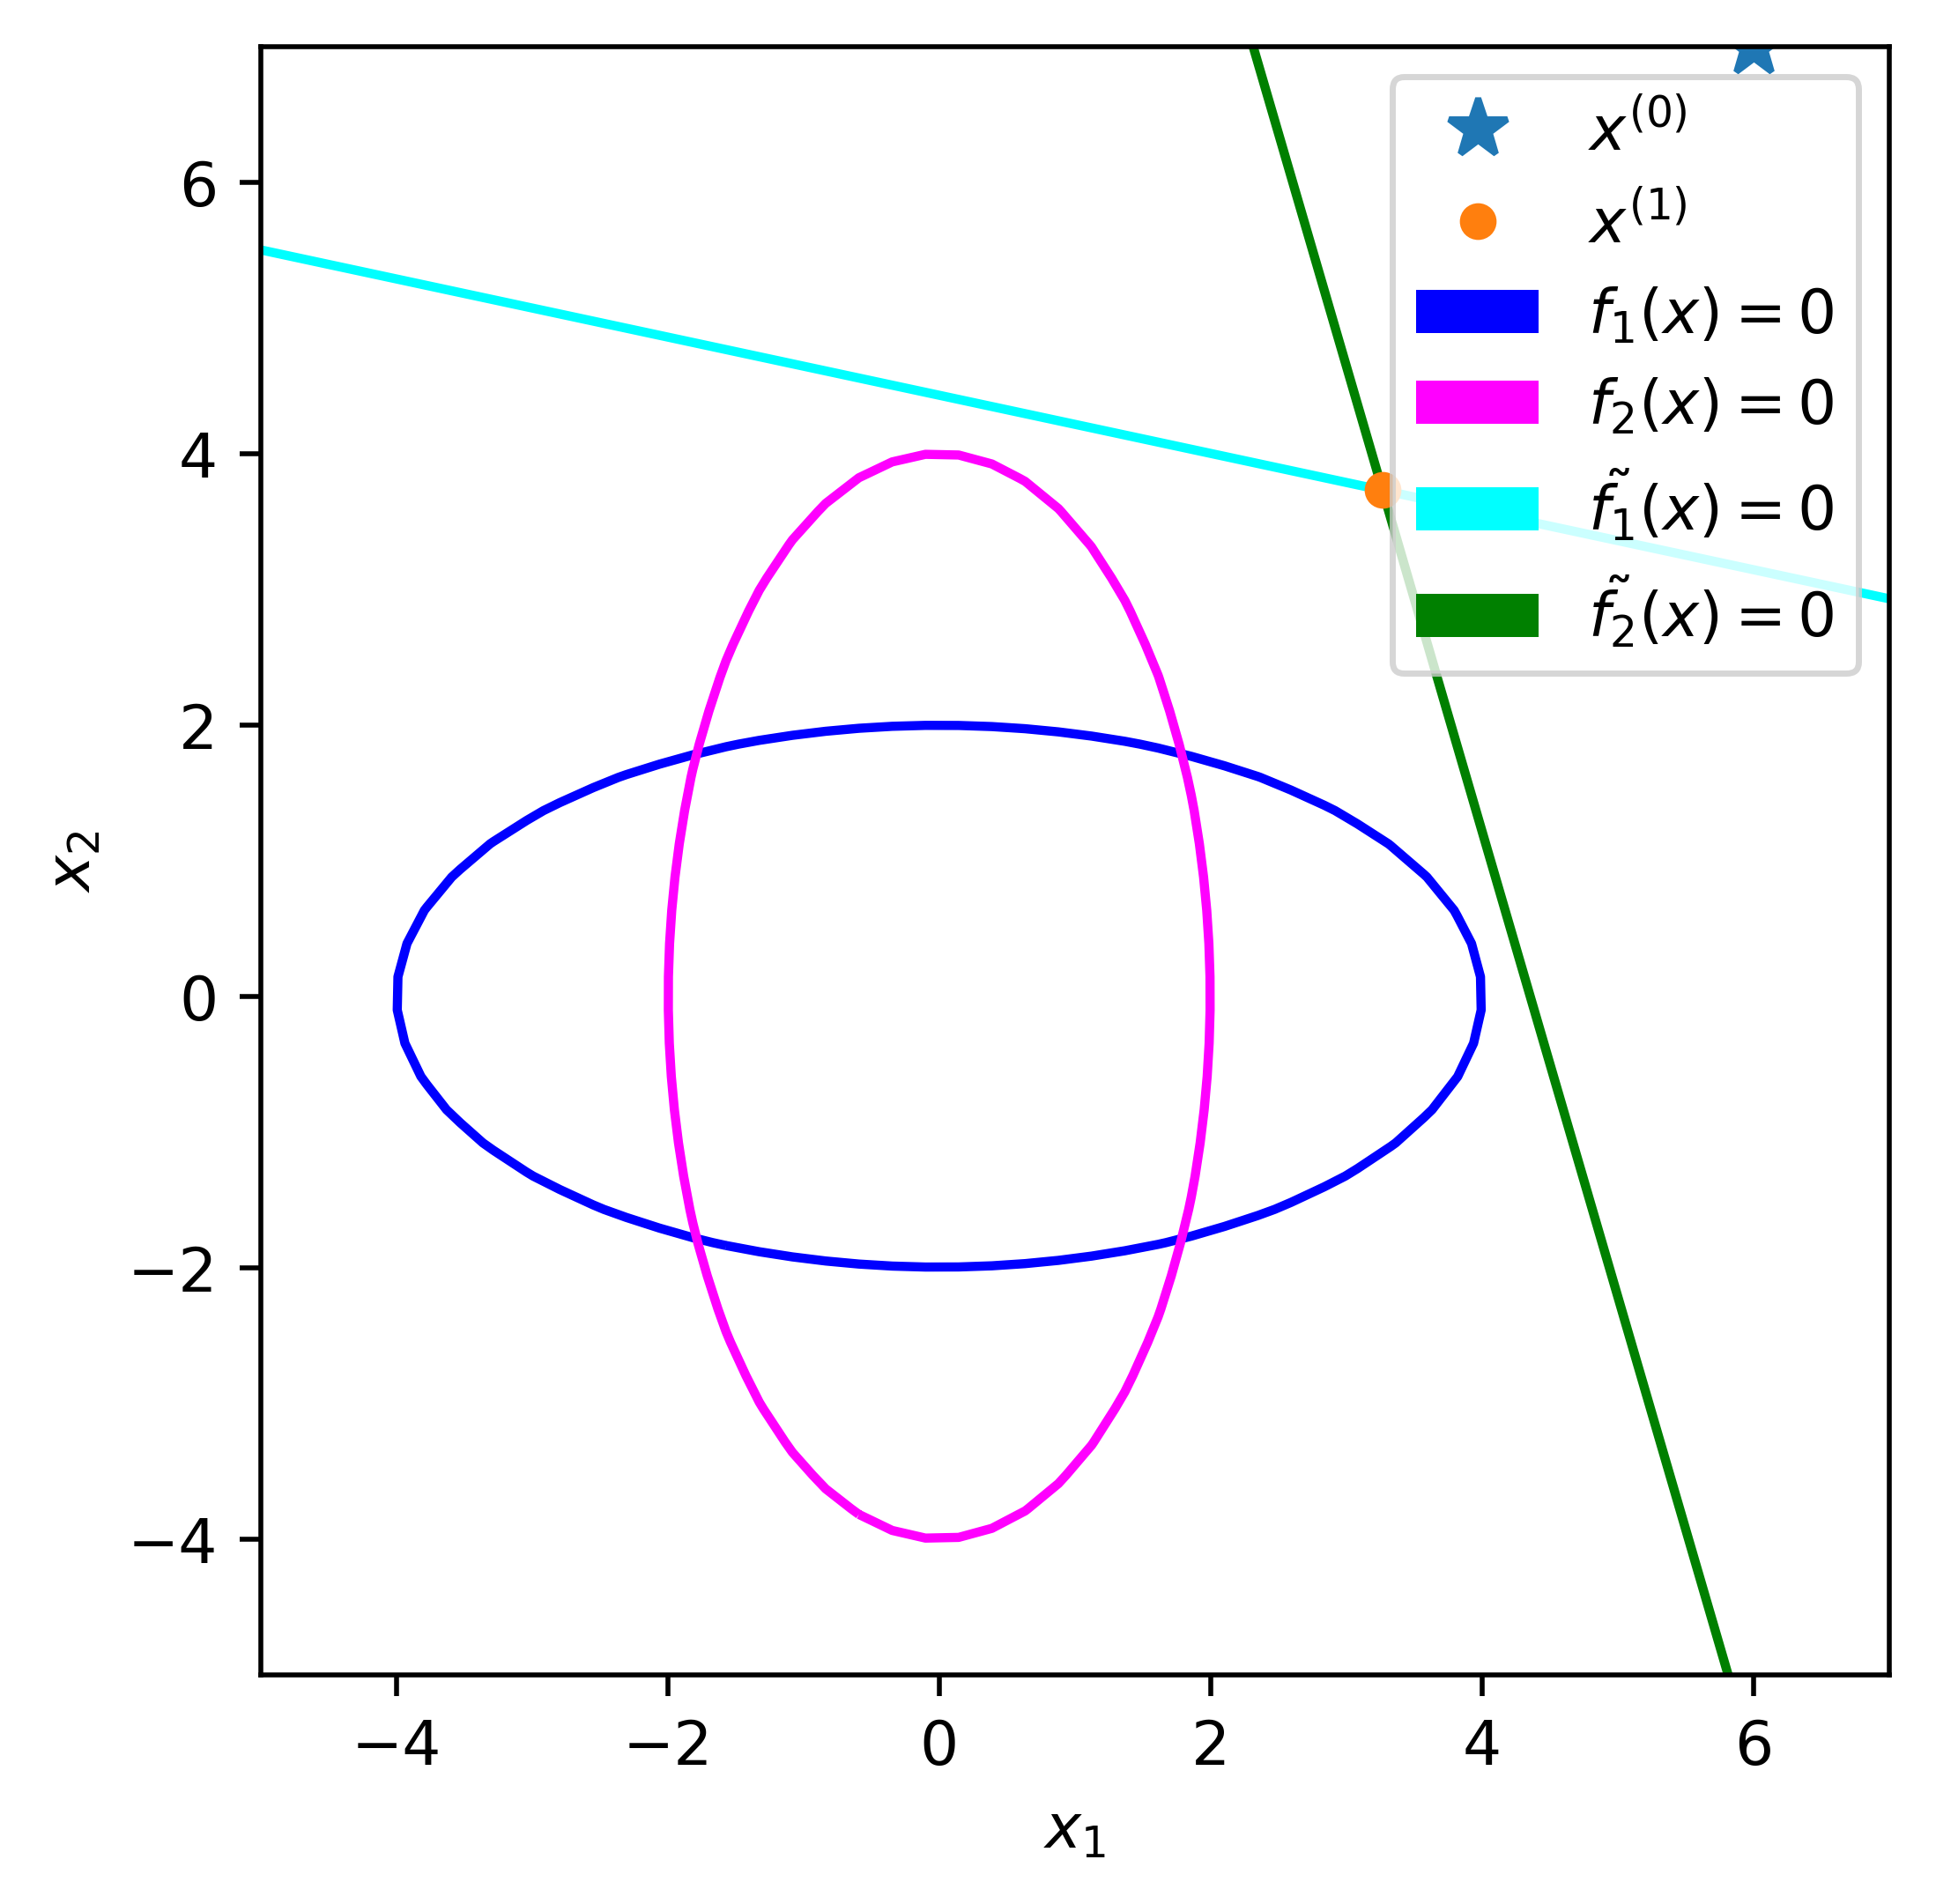
\includegraphics[scale=0.5]{fig0.png}
    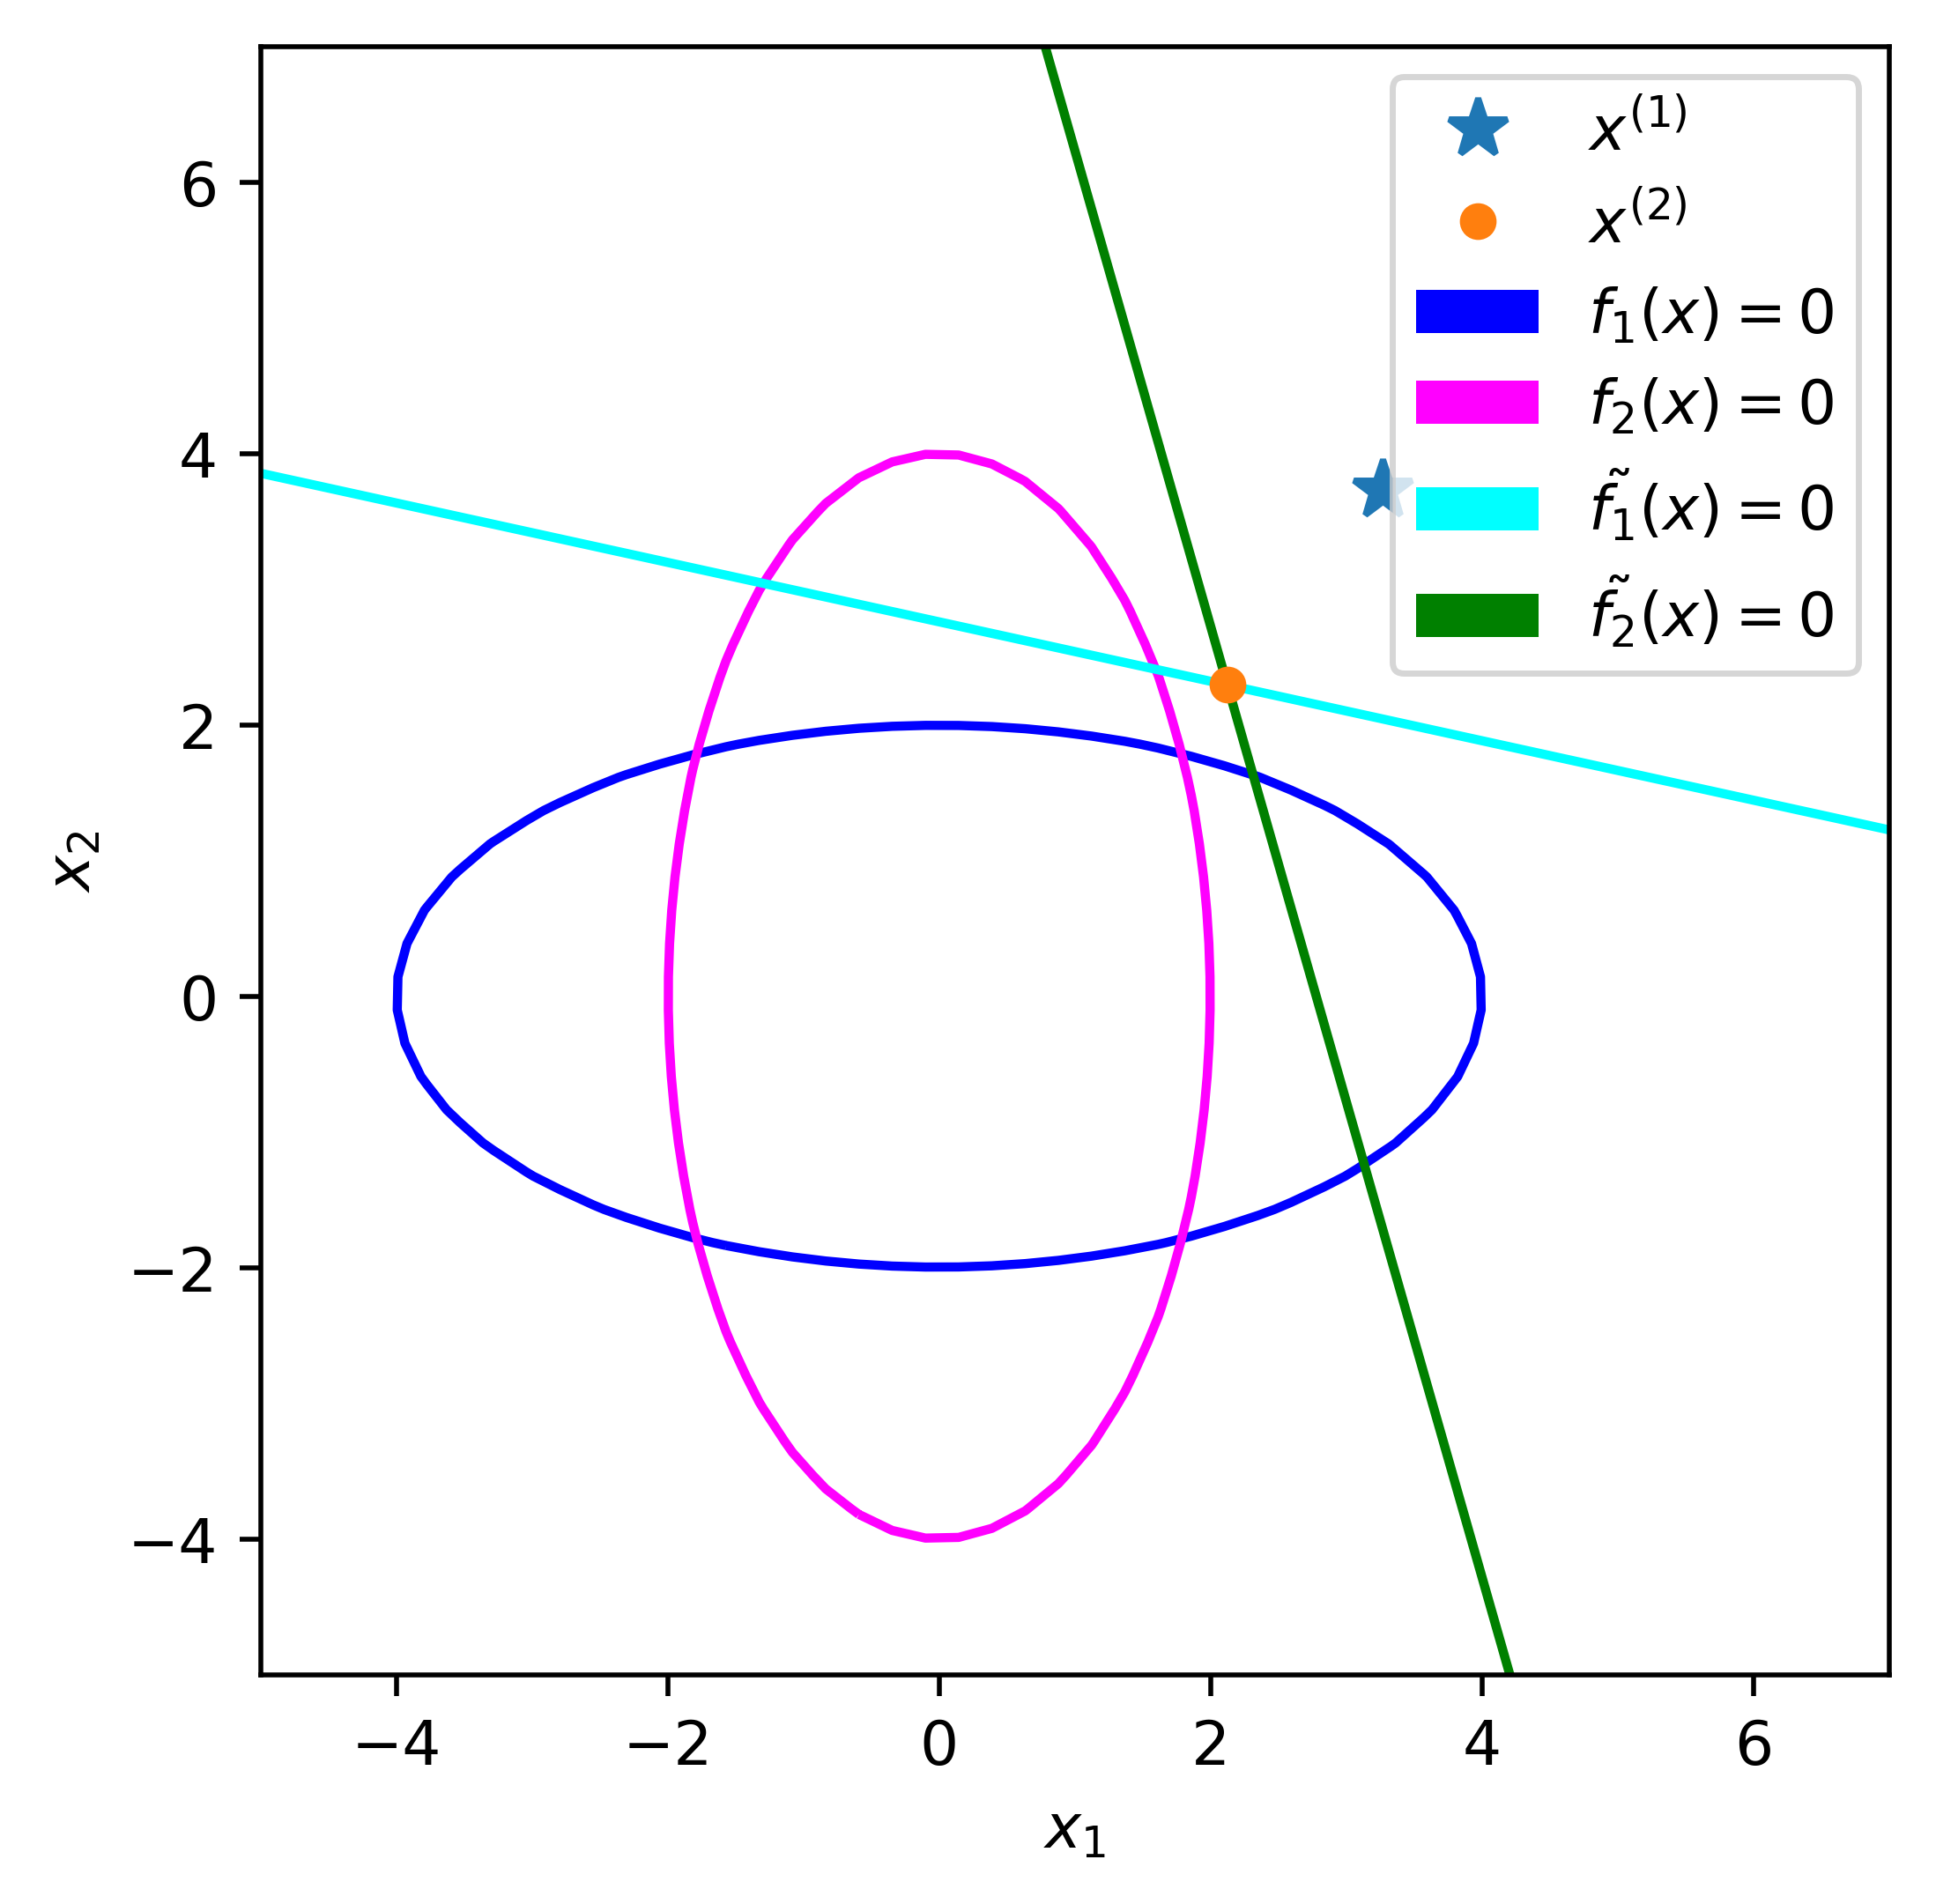
\includegraphics[scale=0.5]{fig1.png}
    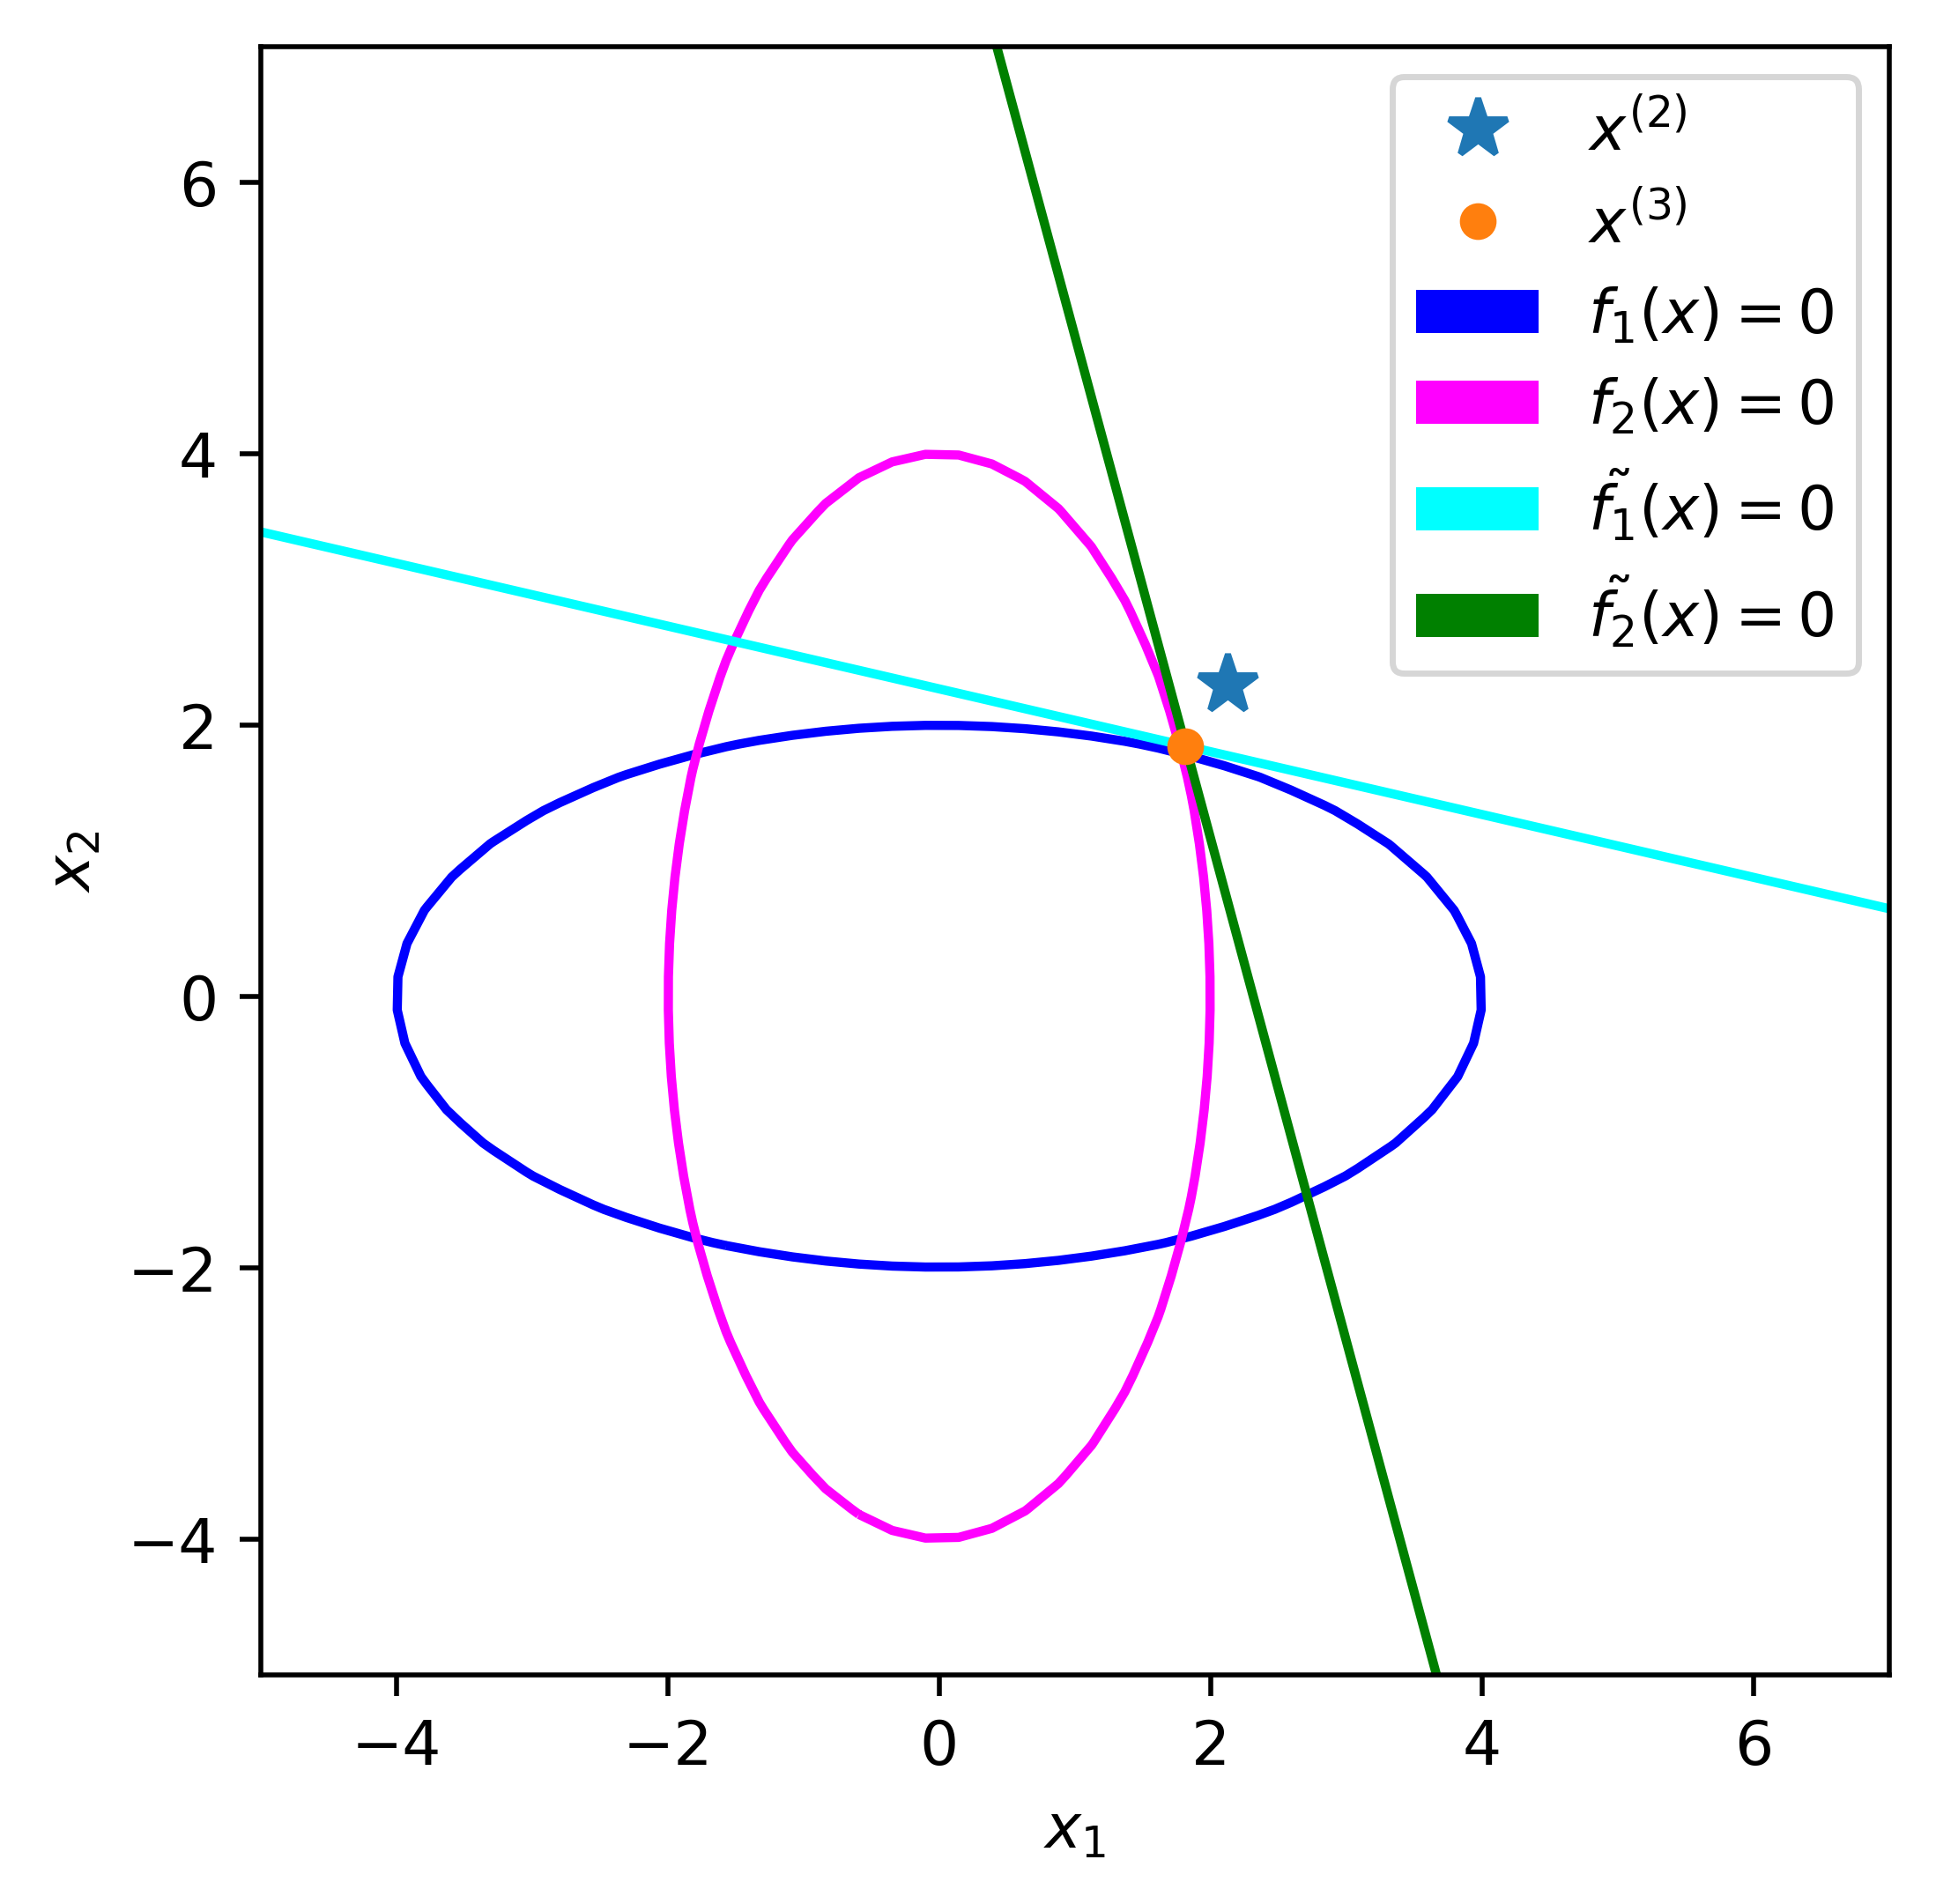
\includegraphics[scale=0.5]{fig2.png}
    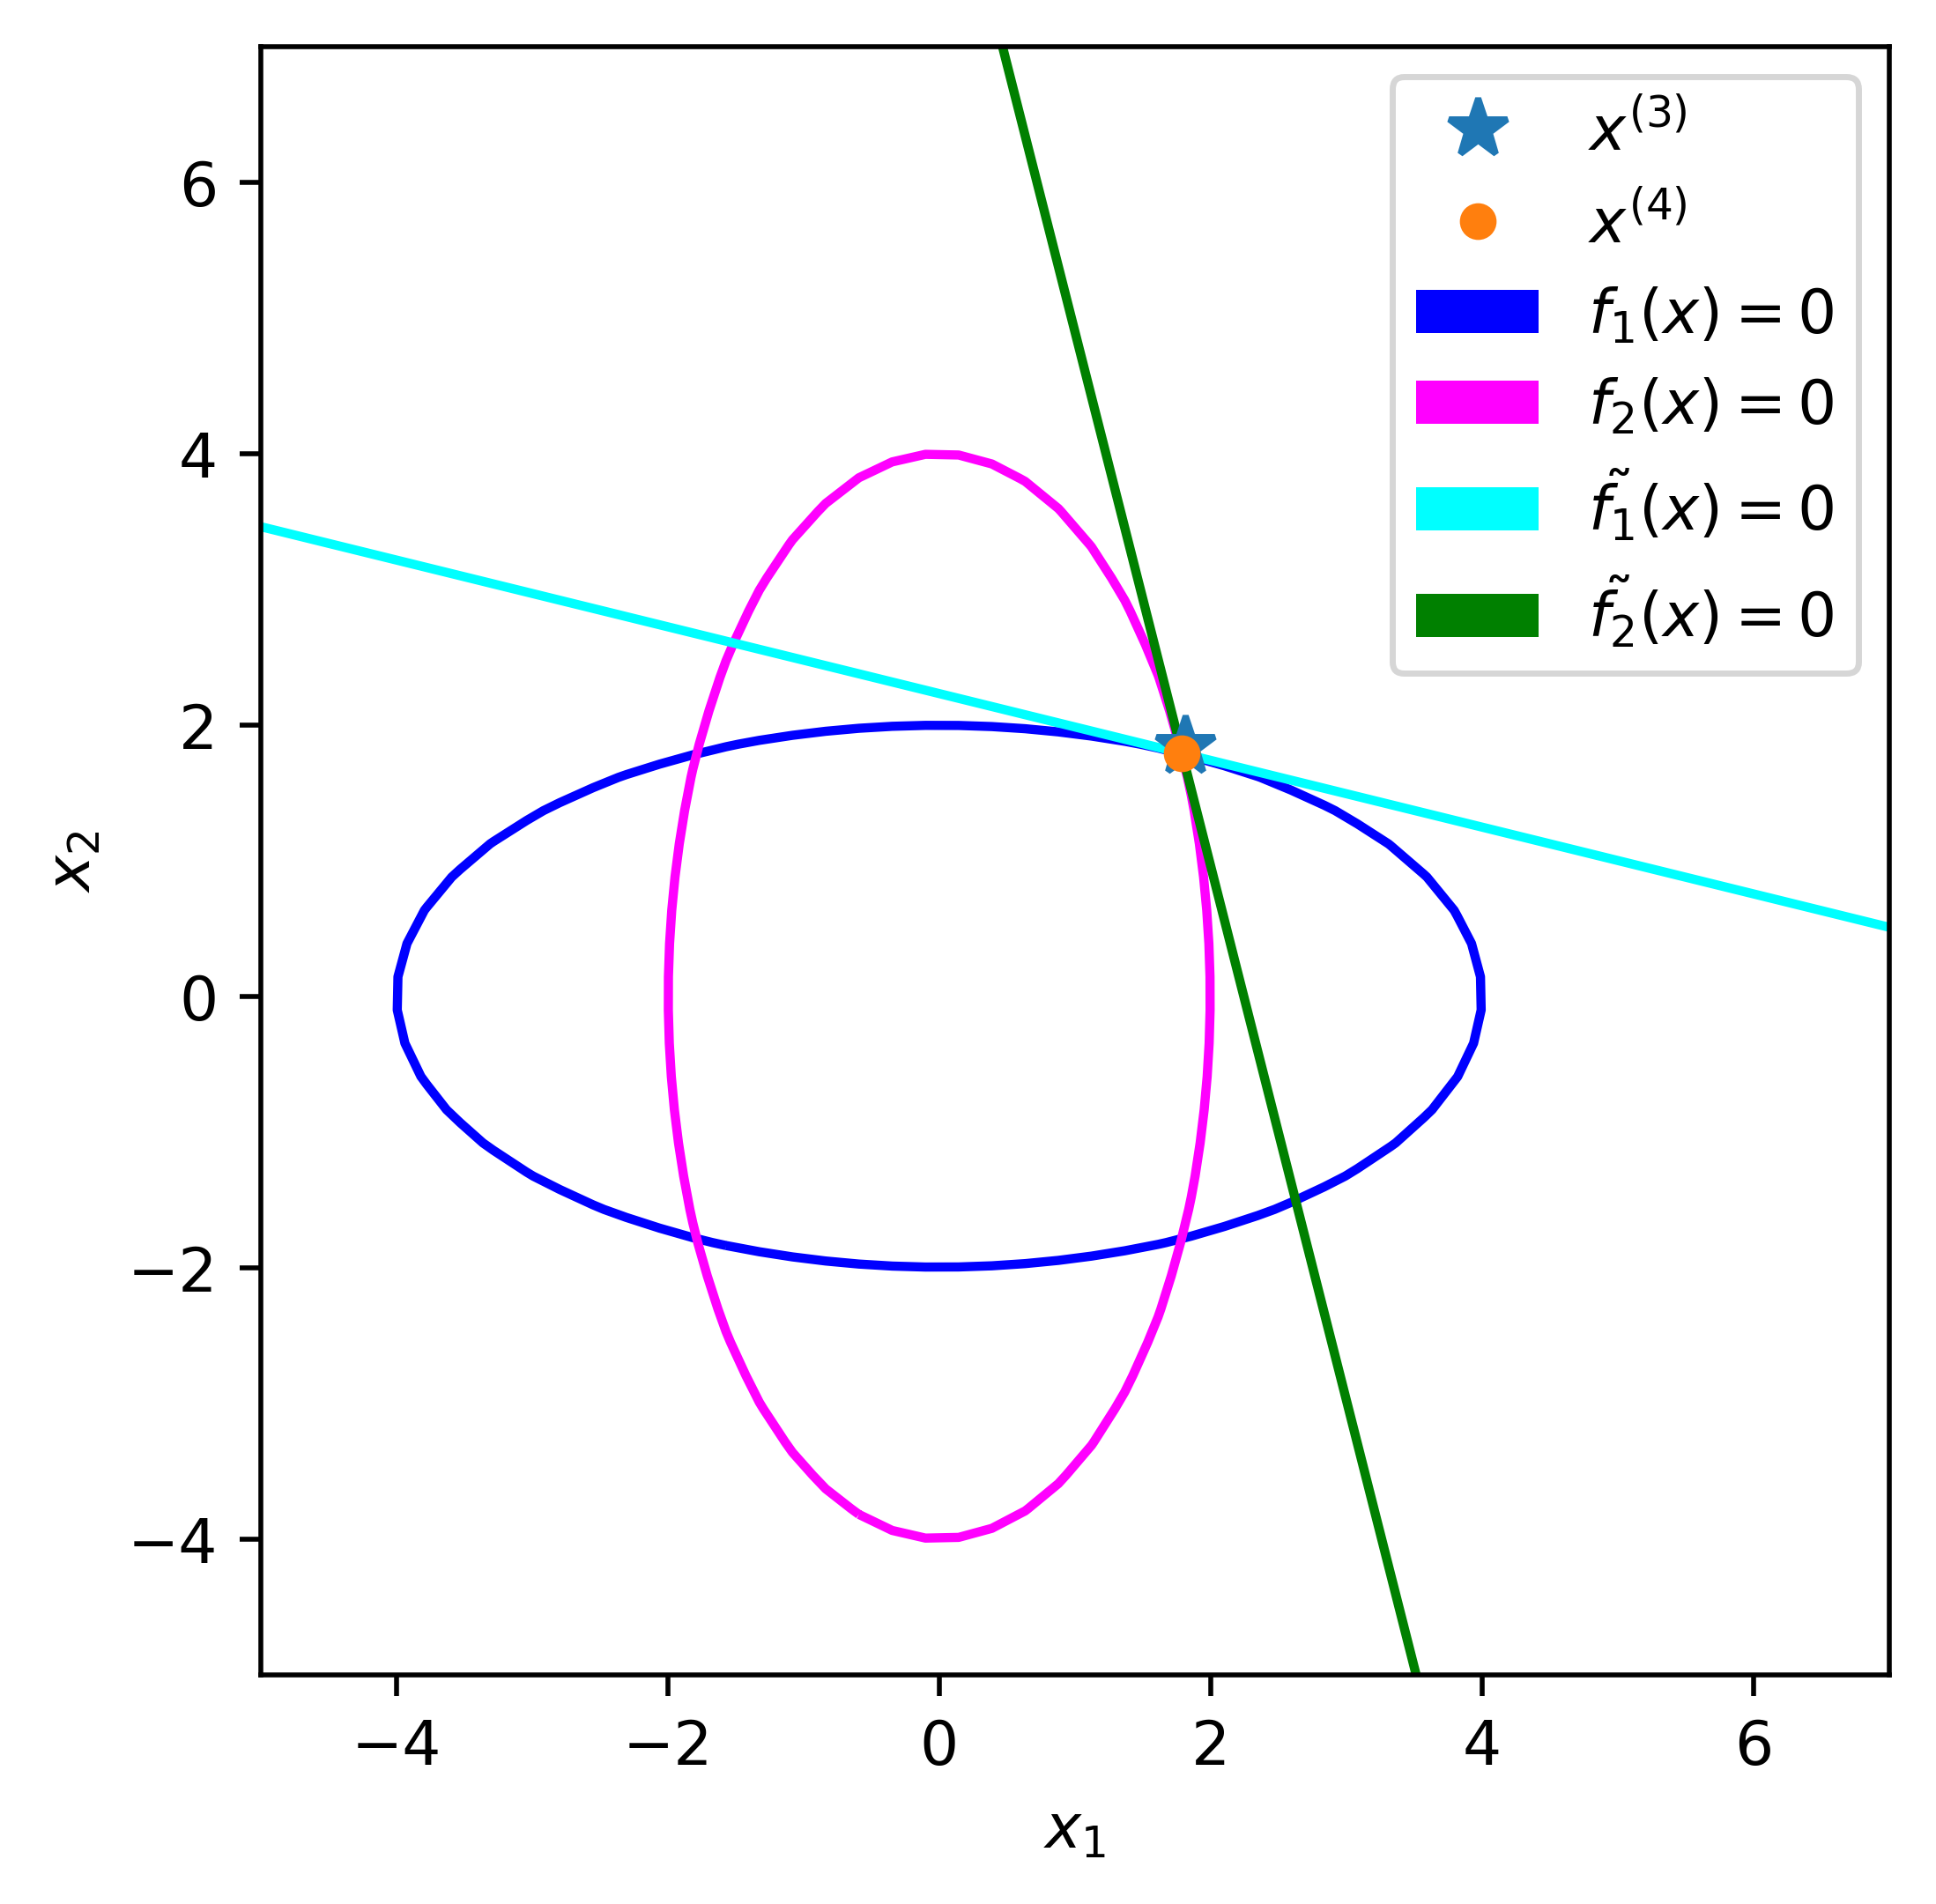
\includegraphics[scale=0.5]{fig3.png}
    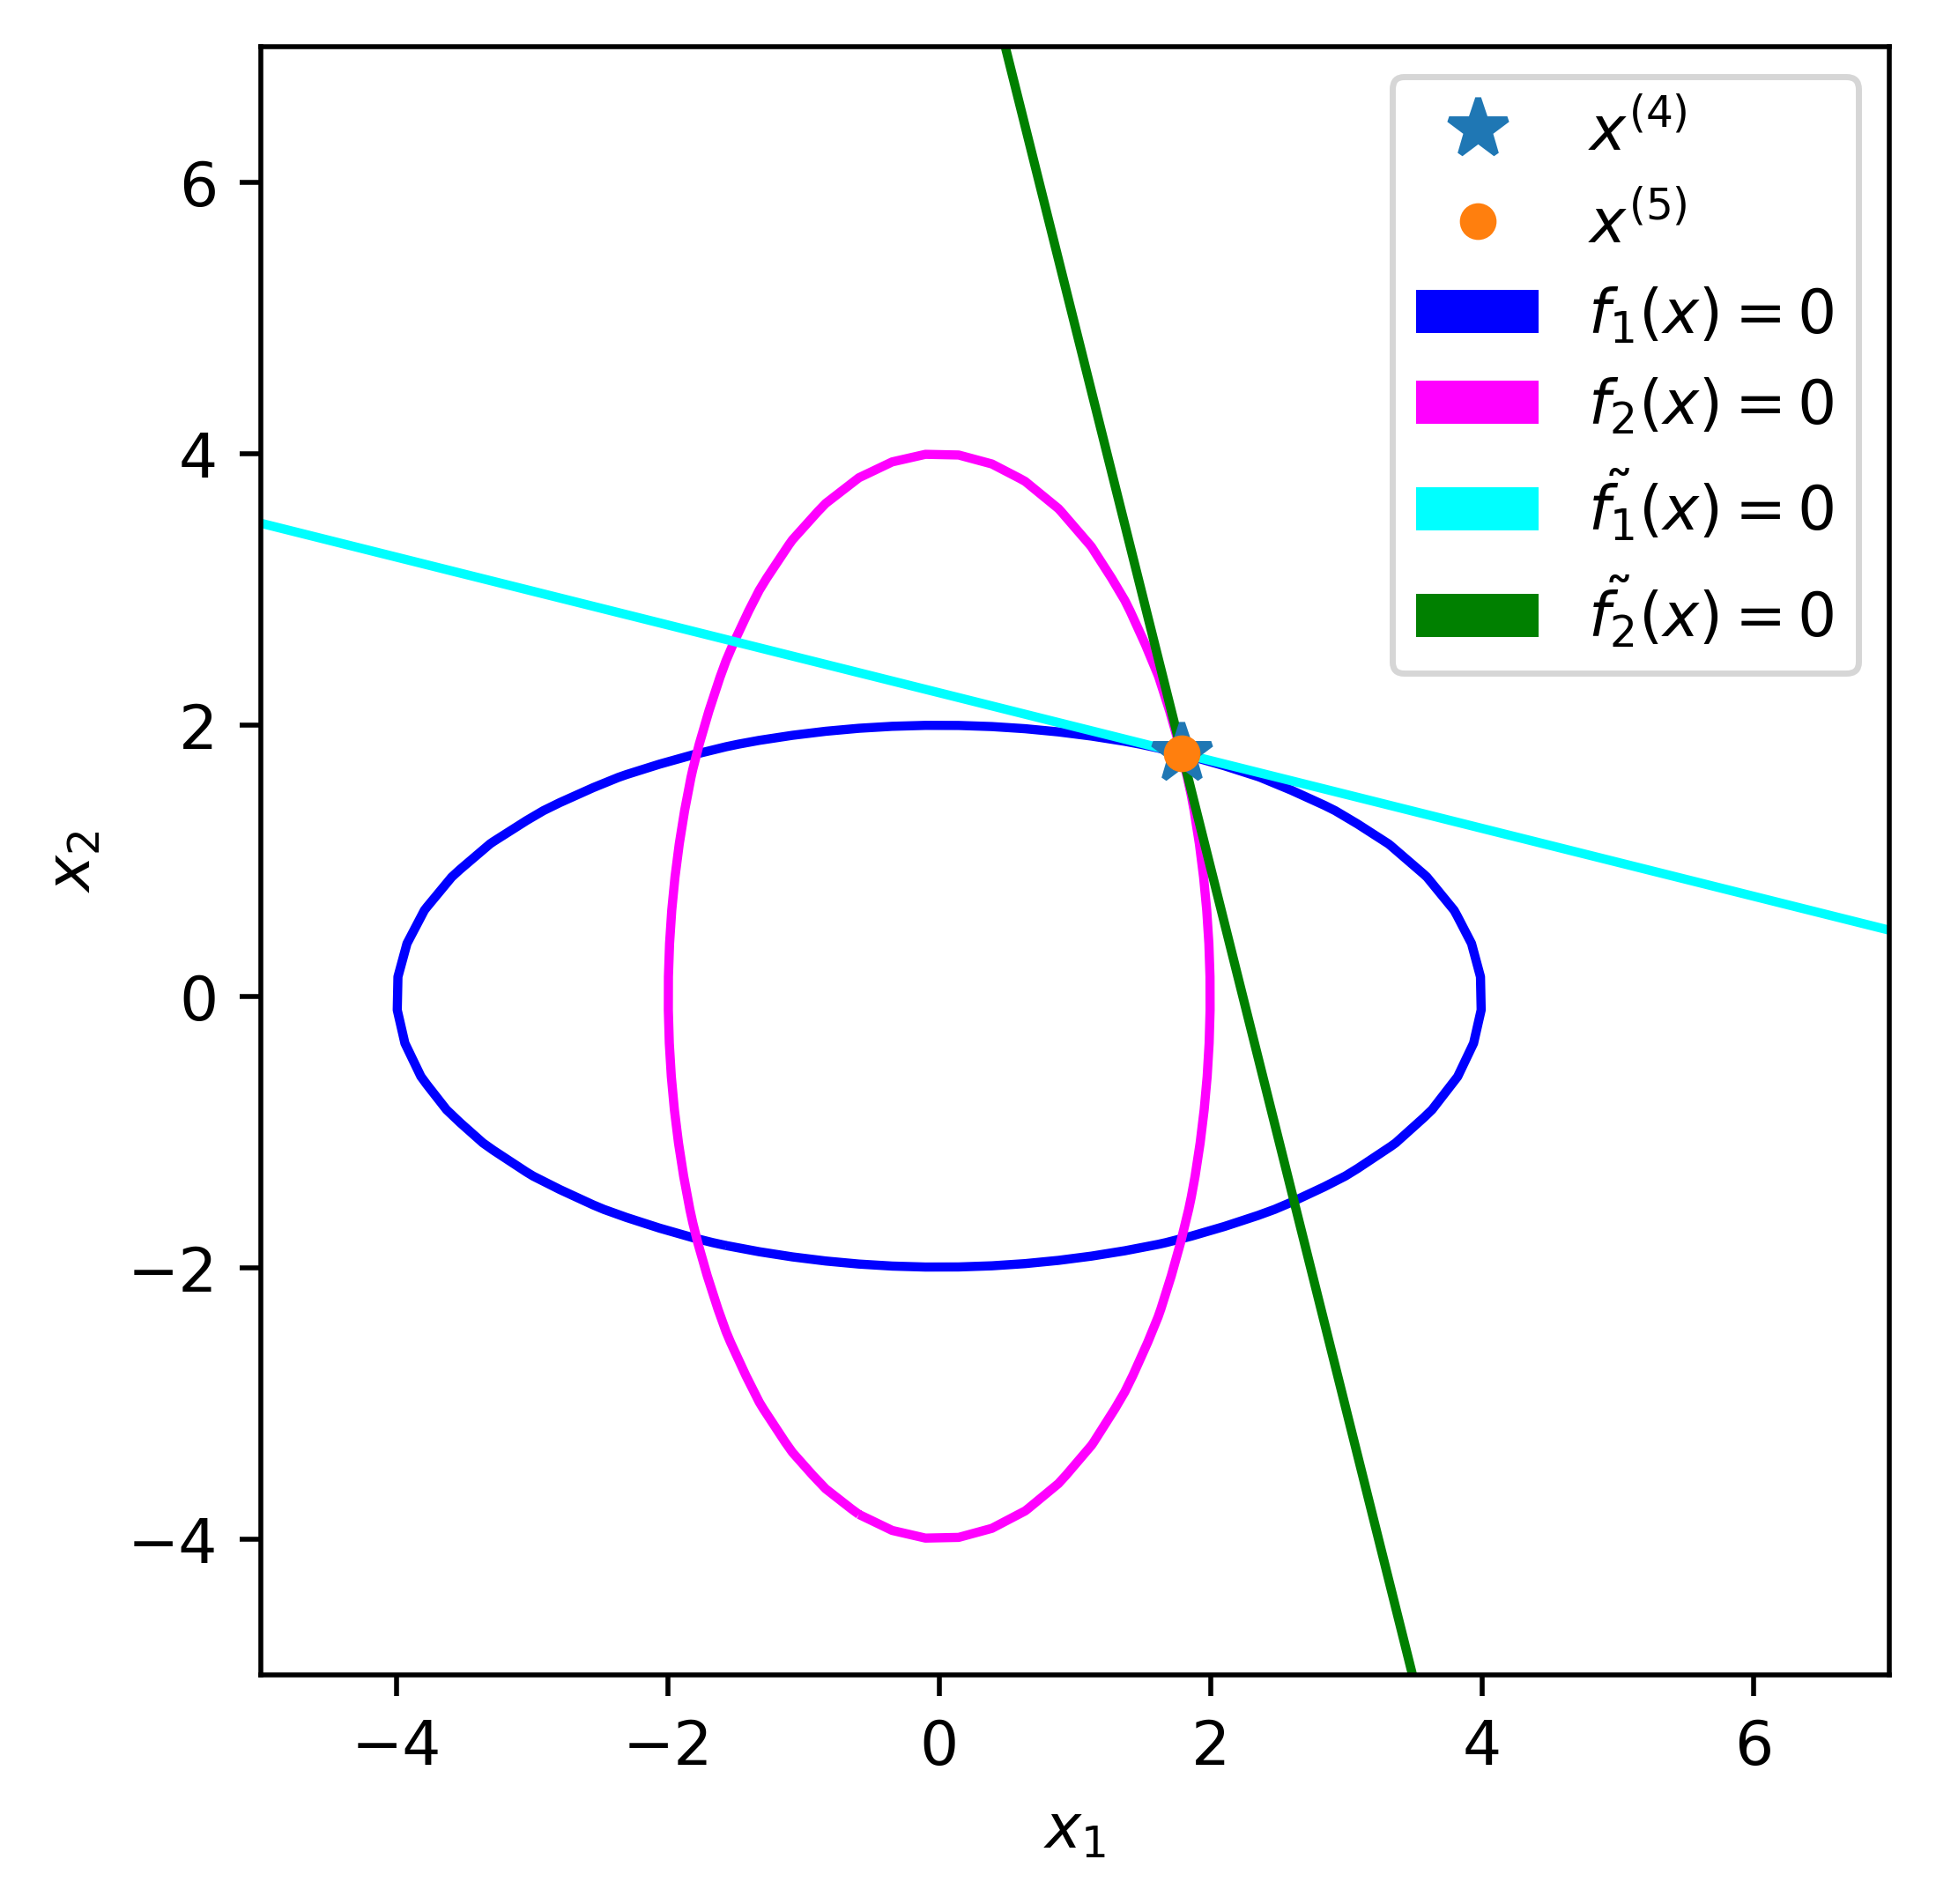
\includegraphics[scale=0.5]{fig4.png}
    \caption{This figure shows the sequence of plots for $x^{(0)}, \cdots, x^{(4)}$ with $x^{(k)}$ as the current Newton iterate and $x^{(k + 1)}$ as the next Newton iterate along the conics and their respective linearized curves.}
    \end{figure*}
\end{enumerate}

\end{document}